\documentclass[11pt,letterpaper]{article}
\usepackage[margin=2.2cm,headheight=15pt]{geometry}
\usepackage[T1]{fontenc}
\usepackage[utf8]{inputenc}
\usepackage[spanish,es-tabla]{babel}
\usepackage{tgheros}
\renewcommand{\familydefault}{\sfdefault}
\usepackage{microtype,graphicx,booktabs,array,longtable,ragged2e,setspace}
\usepackage{csquotes,caption}
\usepackage[backend=biber,style=apa]{biblatex}
\addbibresource{fuentes.bib}
\addbibresource{../citas.bib}
\usepackage{tikz}
\usetikzlibrary{arrows.meta,positioning,calc}
\usepackage{listings,xcolor,fancyhdr,hyperref}
\definecolor{azul}{HTML}{444444}
\definecolor{critico}{HTML}{A43F35}
\definecolor{suave}{HTML}{F3F3F3}
\hypersetup{hidelinks,pdftitle={Escanea y Entra: Plan integral de desarrollo y PERT}}
\newcolumntype{P}[1]{>{\RaggedRight\arraybackslash}p{#1}}
\newcommand{\tablenote}[1]{\par\smallskip{\footnotesize\textit{Nota.} #1\par}}
\newcommand{\figurenote}[1]{\tablenote{#1}}
\newif\ifplantel
\newcommand{\tescha}{\ifplantel TESCHA\else Tecnológico de Estudios Superiores de Chalco (TESCHA)\global\planteltrue\fi}
\newcommand{\pagina}[1]{\clearpage\section{#1}}
\setstretch{1.15}
\setlength{\parindent}{1.27cm}
\setlength{\parskip}{0.15em}
\pagestyle{fancy}\fancyhf{}
\fancyhead[L]{\small ESCANEA Y ENTRA}
\fancyhead[R]{\small Plan integral de desarrollo}
\fancyfoot[C]{\thepage}
\lstset{basicstyle=\ttfamily\footnotesize,backgroundcolor=\color{suave},frame=single,rulecolor=\color{gray!30},breaklines=true,columns=fullflexible,keepspaces=true,showstringspaces=false,extendedchars=true}

\setcounter{tocdepth}{2}
\makeatletter
\renewcommand{\l@section}[2]{%
  \ifnum\c@tocdepth>\z@
    \addpenalty\@secpenalty\addvspace{0.8em}%
    \begingroup
      \parindent\z@\rightskip\@pnumwidth\parfillskip-\@pnumwidth
      \leavevmode\normalfont #1\hfill\hb@xt@\@pnumwidth{\hss #2}\par
    \endgroup
  \fi}
\renewcommand{\l@subsection}[2]{\@dottedtocline{2}{1.5em}{0em}{\hspace*{1.5em}#1}{#2}}
\renewcommand{\tableofcontents}{%
  \begin{center}\bfseries\contentsname\end{center}\vspace{0.6em}%
  \begingroup\setstretch{1.5}\let\numberline\@gobble\@starttoc{toc}\endgroup}
\makeatother

\begin{document}
\pagenumbering{gobble}
\begin{titlepage}
\thispagestyle{empty}
\noindent
\includegraphics[height=1.7cm]{../img/tescha_logo.png}\hfill
\includegraphics[height=1.7cm]{../img/logo_sitemas.png}
\vspace{1.6cm}
\begin{center}
{\Large\bfseries Escanea y Entra\par}
\vspace{0.6cm}
{\LARGE\bfseries Plan integral del proyecto\par}
\vspace{0.5cm}
{\large Alcance, arquitectura, código disponible, dependencias, PERT y ruta de desarrollo\par}
\vspace{1.3cm}
Juan Esteban Anzures Campos\\
Daniel Arellano Palacios\\
Ian Alexis Flores Martínez\\
Miguel Ángel Jurado Delgadillo\\
Juan Fernando Reyes Arguello\\
Bryan Uriel Villegas Raymundo
\vspace{1cm}

Ingeniería en Sistemas Computacionales\\
Tecnológico de Estudios Superiores de Chalco
\vfill
Documento de consolidación técnica y de gestión\\
Corte de revisión: 13 de noviembre de 2026\\
Versión 1.3
\end{center}
\end{titlepage}
\pagenumbering{arabic}
\tableofcontents
\pagina{Propósito y resumen del proyecto}
Este documento reúne la propuesta de investigación, la planeación de gestión y el código disponible de Escanea y Entra, proyecto orientado a evaluar el control de acceso peatonal del \tescha{}. Su finalidad es ofrecer al equipo una guía verificable de qué se quiere construir, qué existe, qué depende de qué y en qué orden desarrollar, probar y entregar el sistema.

El problema de investigación es la falta de evidencia local sobre la duración de la validación de estudiantes, la longitud de la fila y las incidencias de identidad. Se propone un prototipo de torniquete a escala que lea un QR dinámico desde el celular, consulte un servidor, registre la decisión y habilite el paso cuando corresponda. La evaluación compara una línea base con la observación durante un piloto en un acceso del turno vespertino. Este diseño antes-después se apoya en la base metodológica del proyecto \parencite{hernandezsampieri2014metodologia,campbellstanley1963,cranmer2017pretestposttest}.

La documentación delimita la solución operativa al QR. El reconocimiento facial constituye una prueba de concepto para explorar alternativas y producir evidencia de banco. Su existencia no cambia por sí misma el alcance del piloto. NFC aparece en el PERT como parte de una comparación técnica; en las rutas revisadas no se encontró su implementación.

\subsection{Resultados de la consolidación}
\begin{itemize}
\item El PERT de referencia es la hoja \textit{PERT Escanea y Entra}, elaborada por el equipo. Contiene 23 actividades, A a W.
\item El cálculo con las estimaciones originales y sin redondeo intermedio produce \textbf{dos rutas críticas} de \textbf{57,83 días hábiles} desde el inicio lógico del proyecto.
\item La suma de las duraciones esperadas de todas las actividades es \textbf{107,83 días-actividad}; no representa la duración transcurrida ni las horas-persona.
\item Hay documentación y código facial, así como 45 intentos históricos y 24 intentos nuevos del 13 de noviembre. No se verificó una integración operativa de QR, lector, servidor y torniquete.
\end{itemize}

Los antecedentes de control físico mediante QR y de sistemas educativos sustentan la elección del problema y la arquitectura \parencite{kao2011physical,cano2026sistema,alsawi2026qracs}. La aceptación de alternativas biométricas también forma parte de la literatura ya revisada \parencite{rukhiran2023user}.

Las cifras PERT son estimaciones de planeación. Las evidencias revisadas no permiten declarar terminadas todas las tareas con avance, ni calcular un porcentaje global real de ejecución.

\pagina{Fuentes, alcance y criterios de lectura}
\subsection{Material consultado}
\begin{longtable}{P{5.2cm}P{10cm}}
\toprule Fuente & Información utilizada \\ \midrule
\endhead
Documento de investigación e instrumentos de diagnóstico & Problema, objetivos, delimitación, metodología e instrumentos. \\[0.4em]
Informe de Gestión de Proyectos de Software & Gestión, equipo, presupuesto, riesgos y calendario original de octubre de 2026 a enero de 2027. \\[0.4em]
Revisión de objetivos y criterios de aceptación & Decisiones pendientes y criterios de aceptación que todavía requieren acuerdo. \\[0.4em]
Prototipo de reconocimiento facial & Código de registro y reconocimiento, dependencias, 24 intentos del 13 de noviembre y cuatro capturas de las pruebas. \\[0.4em]
Informe de avances del 13 de octubre de 2026 & Código y resultados de 45 intentos, tablas y capturas de una sesión adicional. \\[0.4em]
Plan PERT \textit{Escanea y Entra} & Actividades, dependencias, estimaciones de duración y totales del proyecto. \\ \bottomrule
\end{longtable}
\tablenote{Material del equipo consultado para integrar el estado del proyecto. Las mediciones corresponden a las sesiones indicadas en los resultados.}

\subsection{Qué incluye este documento}
Se integran los objetivos, requisitos, arquitectura propuesta, inventario del código, dependencias técnicas y organizativas, responsabilidades, actividades del PERT, cálculos de precedencia y holgura, rutas críticas, orden de desarrollo, validación, riesgos, costos y entregables. Los instrumentos de encuesta, entrevista y observación permanecen en sus apéndices originales; aquí se explica cuándo se usan y qué producen.

Se distinguen tres niveles de afirmación: \textbf{documentado}, cuando existe una definición o plan; \textbf{implementado en código}, cuando se observa su lógica en los archivos; y \textbf{probado}, cuando hay resultados conservados. Un programa disponible no demuestra que todo el sistema esté instalado o evaluado en campo.

\subsection{Precedencia de las versiones}
El análisis utiliza el plan \textit{PERT Escanea y Entra} del equipo \parencite{pertEquipo}. La hoja \textit{La actividad} contiene una versión parcial con tiempos distintos y no se combina con este plan. El cálculo CPM conserva las estimaciones originales. La fundamentación retoma las fuentes del documento de investigación y del marco teórico.

\pagina{Objetivos, alcance y requisitos}
\subsection{Objetivo general}
Evaluar el efecto de un prototipo basado en QR dinámicos sobre el tiempo de validación y la fila en el acceso piloto, con registro complementario de incidencias de identidad, para aportar evidencia orientativa sobre la conveniencia de ampliar el piloto.

\subsection{Objetivos de trabajo}
\begin{enumerate}
\item Diagnosticar el acceso con encuesta, entrevista y cinco días de observación; documentar acceso, turno, franja horaria y puntos de revisión activos.
\item Definir arquitectura, datos, flujo de autorización, tratamiento de errores y condiciones de operación.
\item Implementar QR dinámicos firmados, validación, registro, lector, controlador y páginas web; integrarlos en un prototipo a escala.
\item Verificar seguridad funcional y desempeño en banco antes de instalarlo.
\item Ejecutar un piloto autorizado, repetir la observación y comparar los indicadores con la línea base.
\item Consolidar la evidencia facial y, si hay equipo y condiciones equivalentes, comparar tecnologías en banco.
\end{enumerate}

\subsection{Límites del producto}
Incluye un acceso, entradas de estudiantes, página con QR, validación en servidor, registro y panel. La revisión manual se mantiene para excepciones y continuidad durante el piloto. No se incluyen torniquetes industriales, todos los accesos, visitantes, salidas ni asistencia por materia. Facial y NFC se contemplan como evaluación separada; incorporarlos a la decisión de apertura exige definir un cambio de alcance.

\subsection{Requisitos funcionales propuestos}
Dar de alta estudiantes autorizados; generar códigos con vigencia; rechazar códigos inválidos, alterados, vencidos o reutilizados; consultar la autorización del estudiante; registrar cada intento con fecha, dispositivo y motivo; abrir una sola vez por autorización; permitir consulta por fecha y estudiante con perfiles de acceso. Los reportes y el padrón deben acordarse con el personal del plantel.

\subsection{Requisitos de calidad}
Medir tiempos y fallos con distintas luces, distancias y brillos. Exigir el rechazo de los casos negativos definidos. La meta de 95\,\% de lecturas exitosas sigue pendiente de acuerdo. Comparar el tiempo total de validación con la línea base, sin reemplazarlo por la inferencia facial.

\pagina{Estado verificable y brechas}
\begin{longtable}{P{3.1cm}P{6.1cm}P{5.6cm}}
\toprule Componente & Evidencia al corte & Pendiente para declararlo completo \\ \midrule
\endhead
Investigación e instrumentos & Secciones del documento y apéndices A a C. & Confirmar revisión y aplicación; conservar datos de campo. \\[0.4em]
Prototipo facial & Registro, reconocimiento, vida, sesiones y análisis en Python. & Calibración ampliada, reproducibilidad y validación en más participantes. \\[0.4em]
Pruebas históricas & 45 intentos guardados en la carpeta de evidencias del 13 de octubre. & Separarlas de nuevas sesiones; completar condiciones y participantes. \\[0.4em]
CSV externo actualizado & 24 intentos del 13 de noviembre, con 11 aciertos. & Revisar las dos falsas aceptaciones y los once falsos rechazos antes de ampliar las pruebas. \\[0.4em]
ESP32-CAM de red & El programa acepta una URL de cámara y el README describe su uso. & Firmware, configuración y evidencia de transmisión desde una placa real. \\[0.4em]
QR, servidor, BD y panel & Definidos en arquitectura, objetivos y PERT. & Código operativo y evidencia del flujo completo en las rutas revisadas. \\[0.4em]
Torniquete y controlador & Planeados en los documentos de gestión. & Ensamble, alimentación, firmware y demostración de apertura segura. \\[0.4em]
NFC & Actividad S del PERT y formato común de resultados propuesto. & Lector, credenciales, programa, protocolo de prueba y resultados. \\[0.4em]
Diagnóstico y piloto & Instrumentos y calendario documentados. & Permisos, registros de aplicación, observación y comparación final. \\ \bottomrule
\end{longtable}
\tablenote{La nota de la hoja que indica avance de A a F se conserva como antecedente; no equivale a cierre validado de las seis actividades. En particular, E no queda demostrado por aceptar una URL, ni F demuestra pruebas con ESP32-CAM.}

Se deberá usar una bitácora por actividad: responsable, estado, evidencia, fecha real de inicio y fin, trabajo restante y bloqueo. El cierre se registra con evidencia revisada, no solo por haber alcanzado la fecha prevista.

\pagina{Arquitectura del sistema y flujo de datos}
\subsection{Solución QR propuesta}
\begin{center}
\begin{tikzpicture}[box/.style={draw=azul,fill=suave,rounded corners,align=center,font=\small,minimum height=1.1cm,text width=3.6cm},arr/.style={-{Latex},thick,azul},node distance=1cm and 1cm]
\node[box](web){Página del estudiante\\QR dinámico};
\node[box,right=of web](cam){ESP32-CAM\\captura y lector QR};
\node[box,right=of cam](esp){ESP32\\control y apertura};
\node[box,below=of cam](srv){Servidor\\valida y autoriza};
\node[box,left=of srv](bd){Base de datos\\padrón e intentos};
\node[box,right=of srv](pan){Panel del personal\\consulta y reportes};
\draw[arr](web)--(cam);\draw[arr](cam)--(esp);
\draw[arrows={Latex-Latex},thick,azul](esp.south)--++(0,-0.35)-|(srv.north);
\draw[arrows={Latex-Latex},thick,azul](srv)--(bd);\draw[arr](srv)--(pan);

\end{tikzpicture}
\end{center}
\figurenote{Arquitectura propuesta, no instalación verificada. La respuesta de autorización vuelve al controlador por el canal de comunicación acordado; el firmware debe distinguir lectura de QR y transmisión de video. La plataforma se fundamenta en las fuentes de ESP32 y ESP32-CAM ya usadas en el marco teórico \parencite{espressif2025esp32,nowroz2025esp32cam}.}

\begin{enumerate}
\item El alumno autenticado solicita un QR con identidad, vigencia e identificador de uso. La regeneración periódica y la combinación de QR con autenticación de un solo uso retoman los antecedentes del proyecto \parencite{nwabuwe2023dynamicqr,chaabani2023labqr,subpratatsavee2015hmac}.
\item El lector decodifica el contenido y el controlador solicita la validación.
\item El servidor verifica integridad, vigencia, habilitación y reutilización, registra la decisión y devuelve un identificador de autorización.
\item El controlador acepta una autorización nueva, libera el mecanismo una vez y registra o confirma la ejecución. Reintentar una petición no debe duplicar el ingreso ni la apertura.
\end{enumerate}
HMAC autentica el mensaje \parencite{krawczyk1997hmac}; evitar su reuso durante la vigencia exige control adicional. HOTP y TOTP aportan las referencias de autenticación de un solo uso basada en contador y tiempo \parencite{mraihi2005hotp,mraihi2011totp}; K debe definir cuál esquema se implementará. Tampoco evita que se preste el celular. Estas condiciones deben quedar en el diseño y en los casos de prueba.

\subsection{Rama facial existente}
Cámara local o URL de video $\rightarrow$ detección $\rightarrow$ vector $\rightarrow$ comparación $\rightarrow$ comprobación de vida cuando está habilitada $\rightarrow$ decisión y CSV. La inferencia se realiza en la computadora; el ESP32-CAM se plantea como fuente de imágenes. No se encontró una interfaz del módulo facial con el servidor de acceso o el mecanismo de apertura.

\pagina{Inventario del código de reconocimiento facial}
\begin{longtable}{P{3.8cm}P{11cm}}
\toprule Archivo & Función observada \\ \midrule
\endhead
\path{comun.py} & Rutas, cámara, motores, vectores, similitud coseno y visualización. SFace usa YuNet y SFace; buffalo\_s y buffalo\_l usan InsightFace. La decisión compara el mejor parecido con el umbral. \\[0.4em]
\path{registrar.py} & Solicita confirmación de consentimiento, captura cinco muestras por defecto y guarda vectores por motor en archivos \texttt{.npy}. Rechaza identificadores inválidos o ya registrados. \\[0.4em]
\path{reconocer.py} & Ejecuta intentos, toma el tiempo, obtiene identidad y aplica vida pasiva, activa o ambas si corresponde. Escribe resultado esperado, obtenido, similitud, tiempo y detalle en CSV. \\[0.4em]
\path{vida.py} & Modelo pasivo y reto activo de giros, parpadeo y retorno al frente; comprueba paralaje y continuidad de identidad. \\[0.4em]
\path{sesion.py} & Guía condiciones con tres combinaciones: SFace sin vida, buffalo\_l sin vida y buffalo\_l con vida pasiva. Permite saltar o terminar pasos. No recorre automáticamente todas las opciones de vida. \\[0.4em]
\path{analizar.py} & Agrupa por tecnología, condición y resultado esperado; calcula aciertos, falsas aceptaciones, falsos rechazos y tiempos. No sustituye un diseño de muestreo. \\[0.4em]
\path{descargar_modelos.py} & Descarga modelos y comprueba hashes SHA-256 definidos en el programa. \\[0.4em]
\path{borrar_datos.py} & Elimina vectores por sujeto o de todos, después de confirmación. No elimina el CSV, por lo que su conservación requiere una regla independiente. \\ \bottomrule
\end{longtable}

Los umbrales actuales del código son 0,363 para SFace y 0,40 para los motores InsightFace; en vida se usa 0,8 para la modalidad pasiva, 20 grados para giros y 0,12 para paralaje. Son parámetros iniciales de la implementación, no desempeño validado para la población del plantel.

El reconocimiento elige el rostro de mayor área cuando hay varios. El registro exige una cara en el motor guía, pero eso no establece una política de acceso para escenas con varias personas. La vida activa aumenta el tiempo de interacción y tiene limitaciones ante videos o máscaras, descritas en el README. Estas condiciones se deben cubrir en la ampliación de pruebas.

\pagina{Dependencias técnicas y operación reproducible}
\subsection{Dependencias declaradas y bloqueadas}
\begin{center}
\begin{tabular}{P{3.8cm}P{3.8cm}P{6.6cm}}
\toprule Componente & Declaración / bloqueo & Uso en el prototipo \\ \midrule
Python & $\geq$ 3.12 & Ejecución de programas. \\
InsightFace & $\geq$ 2.1 / 2.1 & Motores buffalo y modelo de vida pasiva. \\
MediaPipe & $\geq$ 1.1.0 / 1.1.0 & Pose, gestos y parpadeo. \\
NumPy & $\geq$ 2.5.4 / 2.5.4 & Vectores, matrices y similitud. \\
ONNX Runtime & $\geq$ 1.31.0 / 1.31.0 & Ejecución de modelos. \\
OpenCV Python & $\geq$ 5.0.0.93 / 5.0.0.93 & Captura, detección y visualización. \\ \bottomrule
\end{tabular}
\end{center}
\tablenote{Versiones leídas de \texttt{pyproject.toml} y \texttt{uv.lock}; no equivalen a una comprobación del entorno instalado ni se proponen como versiones nuevas para instalar.}

Se requieren una computadora con cámara y entorno gráfico para las ventanas de OpenCV, almacenamiento de modelos y vectores, y conectividad para preparar el entorno. Los motores InsightFace se configuran para CPU en el código. Si se usa cámara de red, se necesita comprobar dirección, transmisión, estabilidad y resolución. Los modelos y sus condiciones de uso se revisan antes de cambiar de un experimento a un despliegue institucional.

\subsection{Secuencia de preparación}
Para reproducir el entorno declarado se recomienda conservar \texttt{uv.lock} y usar \texttt{--locked}, que falla si el archivo requiere actualización en vez de resolverlo silenciosamente \parencite{uvDocs}. Los siguientes comandos se ejecutan desde la carpeta del prototipo de reconocimiento facial.
\begin{lstlisting}
uv sync --locked
uv run --locked descargar_modelos.py
uv run --locked registrar.py --sujeto s02
uv run --locked sesion.py --sujeto s02
uv run --locked analizar.py
\end{lstlisting}
Antes de registrar se verifica el consentimiento y el código del participante. No se deben sobrescribir ni sumar respaldos con intentos coincidentes. Cada sesión nueva requiere registrar cámara, equipo, configuración y condiciones.

\subsection{Dependencias todavía por seleccionar}
Las dependencias del servidor, del panel y del firmware QR todavía no están definidas en la evidencia revisada. Lenguaje del servidor, motor de base de datos, herramientas web, librería de decodificación QR y mecanismo de comunicación entre placas permanecen por confirmar. La actividad K debe fijar estas decisiones; las dependencias del prototipo facial no cubren esos módulos.

\pagina{Evidencia histórica y medición}
Esta sección presenta los 45 intentos de calibración del 13 de octubre de 2026. Se analizan por separado de los 24 intentos del 13 de noviembre, descritos en la sección siguiente. No se contabilizan registros duplicados del respaldo. Las capturas de detección y parpadeo de una sesión adicional son evidencia visual separada.

\begin{center}
\begin{tabular}{P{2.5cm}P{4.1cm}rrr}
\toprule Vida & Condición histórica & Intentos & Correctos & Media (ms) \\ \midrule
Activa & Rostro real & 5 & 4 & 5520,6 \\
Ambas & Rostro real & 5 & 5 & 6008,9 \\
Ambas & Fotografía de s01 & 10 & 10 & 245,9 \\
Ambas & Otras personas & 5 & 5 & 234,2 \\
Pasiva & Foto en celular & 10 & 10 & 207,1 \\
Pasiva & Rostro real & 10 & 9 & 216,4 \\
\midrule
Total & Motor buffalo\_l & 45 & 43 & -- \\ \bottomrule
\end{tabular}
\end{center}
\tablenote{Fuente local histórica. Las medias incluyen los intentos correctos e incorrectos de cada grupo. Los rechazos antes del reto activo pueden ser mucho más breves que una aceptación con reto.}

Hubo 18 aceptaciones correctas en los 20 intentos que debían aceptarse y 25 rechazos correctos en 25 intentos que debían rechazarse. Los dos falsos rechazos corresponden al encuadre en vida pasiva y al parpadeo en vida activa. Los 43 aciertos de 45 describen esta calibración y no estiman por sí solos el desempeño poblacional.

Todos los intentos están asociados al código s01; la etiqueta de otras personas no permite contar individuos distintos. No hay ensayos históricos de QR o NFC en ese archivo, ni una comparación completa entre los tres motores.

\subsection{Tres tiempos que deben mantenerse separados}
\begin{itemize}
\item \textbf{Procesamiento de banco:} desde la tecla de intento hasta la decisión; incluye el reto si es activo, pero no la colocación inicial ni la transmisión previa del cuadro.
\item \textbf{Validación de acceso:} desde que la persona llega al punto de revisión hasta que lo cruza; es el indicador comparable con la revisión manual.
\item \textbf{Espera y fila:} efecto del flujo y del número de puntos activos; se obtiene por observación, no del CSV facial.
\end{itemize}
Para la actividad S se necesita el mismo inicio y fin del cronometraje, participantes y condiciones comparables. No se puede concluir que una tecnología es más rápida comparando inferencia local con cruce completo de otra.

\pagina{Resultados de las pruebas del 13 de noviembre de 2026}
La sesión del 13 de noviembre contiene \textbf{24 intentos}, registrados entre las 15:56:25 y las 16:03:26. Todos utilizan \texttt{buffalo\_l} con vida \texttt{ambas}. Se mantienen separados de los 45 intentos de octubre porque son sesiones y condiciones distintas. Los resultados siguientes proceden de las etiquetas del archivo; hace falta revisar su correspondencia con el protocolo antes de atribuir cada error al algoritmo.

\subsection{Resumen de decisiones y tiempos}
\begin{center}\small\singlespacing
\begin{tabular}{P{2.7cm}rrrrrrrr}\toprule Condición & $n$ & Aciertos & \% & FR & FA & Media & Mediana & Máx. \\ \midrule
Foto en celular & 8 & 7 & 87,5 & 0 & 1 & 715,4 & 222,8 & 4100,7 \\
Luz normal & 16 & 4 & 25,0 & 11 & 1 & 3013,4 & 255,1 & 12021,2 \\
\bottomrule\end{tabular}
\end{center}
\tablenote{Tiempos en milisegundos. FR = falsos rechazos; FA = falsas aceptaciones, incluyendo aceptación con identidad distinta de la esperada. Fuente: \texttt{pruebas-2026-11-13.csv}. El resumen de análisis se incluye en los anexos CSV.}

Hay \textbf{11 aciertos en 24 intentos} (45,8\,\%). En luz normal, el archivo contiene 16 intentos que debían aceptarse: cuatro aceptaciones con identidad correcta, once decisiones de rechazo y una aceptación con otra identidad. Los cuatro intentos de s01 incluyen dos aciertos; los doce de s03 incluyen dos. La condición foto en celular reúne ocho intentos de s01: siete rechazos y una aceptación etiquetada como incorrecta.

\subsection{Casos que requieren revisión}
\begin{itemize}
\item \textbf{Foto aceptada, 16:00:10.} El archivo etiqueta el caso como \texttt{foto\_celular}, esperado rechazo, pero registra aceptación de s01 con similitud 0,7808, vida pasiva 1,00 y paralaje 0,26/0,26. El tiempo es 4100,7 ms. Se debe comprobar qué se presentó y reproducir la condición; no se omite este caso por haber siete rechazos correctos.
\item \textbf{Identidad distinta, 16:02:00.} El sujeto esperado es s03 y se registra aceptación como s04, similitud 0,7947, vida pasiva 1,00, paralaje 0,20/0,24 y 12021,2 ms. Dos capturas posteriores conservan esta decisión en pantalla; documentan el mismo resultado, no dos falsas aceptaciones adicionales.
\item \textbf{Rechazos de casos de aceptación.} Se registran fallos de giro a derecha e izquierda, rostro cortado y ocho rechazos de identidad con el detalle vacío. El CSV no permite fijar la causa de esos ocho casos. Conviene revisar etiquetas, vectores registrados, encuadre y configuración antes de repetir las pruebas.
\end{itemize}

Las dos FA no deben dividirse entre un único denominador: la aceptación en foto es 1/8 de los casos de rechazo; la confusión es 1/16 de los casos de aceptación. FR es 11/16 (68,75\,\%). Las medias y medianas incluyen rechazos tempranos, de modo que una mediana breve no implica que el acceso completo sea rápido.

\pagina{Bitácora de intentos y archivos CSV anexos}
Se conserva cada registro de noviembre sin corregir identidades ni etiquetas. La tabla resume sus campos principales; los CSV entregados mantienen también tecnología, resultado esperado, similitud y detalle. Luz normal tiene resultado esperado de aceptación; foto, de rechazo.
\begin{center}\small\singlespacing
\begin{tabular}{rlclllrr}\toprule N.º & Hora & Sujeto & Condición & Resultado & Identidad & ms & OK \\ \midrule
1 & 15:56:25 & s01 & Luz normal & Rechazo vida & s01 & 7206,3 & 0 \\
2 & 15:58:23 & s01 & Luz normal & Rechazo vida & s01 & 225,3 & 0 \\
3 & 15:58:33 & s01 & Luz normal & Acepta & s01 & 7164,1 & 1 \\
4 & 15:58:42 & s01 & Luz normal & Acepta & s01 & 3423,0 & 1 \\
5 & 15:59:31 & s01 & Foto & Rechazo vida & s01 & 154,0 & 1 \\
6 & 15:59:36 & s01 & Foto & Rechazo vida & s01 & 330,0 & 1 \\
7 & 15:59:37 & s01 & Foto & Rechazo vida & s01 & 212,4 & 1 \\
8 & 15:59:38 & s01 & Foto & Rechazo vida & s01 & 268,9 & 1 \\
9 & 15:59:39 & s01 & Foto & Rechazo vida & s01 & 226,2 & 1 \\
10 & 16:00:10 & s01 & Foto & Acepta & s01 & 4100,7 & 0 \\
11 & 16:00:15 & s01 & Foto & Rechazo vida & s01 & 211,7 & 1 \\
12 & 16:00:16 & s01 & Foto & Rechazo vida & s01 & 219,3 & 1 \\
13 & 16:01:21 & s03 & Luz normal & Acepta & s03 & 5915,2 & 1 \\
14 & 16:01:41 & s03 & Luz normal & Rechazo vida & s04 & 5245,2 & 0 \\
15 & 16:02:00 & s03 & Luz normal & Acepta & s04 & 12021,2 & 0 \\
16 & 16:02:57 & s03 & Luz normal & Rechazo & -- & 212,4 & 0 \\
17 & 16:02:59 & s03 & Luz normal & Rechazo & -- & 204,9 & 0 \\
18 & 16:03:03 & s03 & Luz normal & Rechazo & -- & 209,6 & 0 \\
19 & 16:03:09 & s03 & Luz normal & Rechazo & -- & 199,8 & 0 \\
20 & 16:03:11 & s03 & Luz normal & Rechazo & -- & 207,8 & 0 \\
21 & 16:03:13 & s03 & Luz normal & Rechazo & -- & 284,9 & 0 \\
22 & 16:03:14 & s03 & Luz normal & Rechazo & -- & 206,3 & 0 \\
23 & 16:03:15 & s03 & Luz normal & Rechazo & -- & 212,4 & 0 \\
24 & 16:03:26 & s03 & Luz normal & Acepta & s03 & 5275,3 & 1 \\
\bottomrule\end{tabular}
\end{center}
\tablenote{OK reproduce \texttt{correcto}: 1 = decisión correcta según la etiqueta; 0 = incorrecta. Las filas 10 y 15 son las dos FA registradas. El número de fila se añade para lectura y no sustituye la marca de tiempo del CSV.}

\subsection{Archivos que acompañan el documento}
\begin{itemize}
\item \texttt{pruebas-2026-10-13.csv}: 45 registros de la sesión de octubre, sin sumar registros duplicados del respaldo.
\item \texttt{analisis-2026-10-13.csv}: seis grupos con conteos, aciertos, FR, FA, media, mediana y máximo.
\item \texttt{pruebas-2026-11-13.csv}: 24 registros de la sesión de noviembre.
\item \texttt{analisis-2026-11-13.csv}: dos grupos con las mismas métricas, sin mezclar las sesiones.
\end{itemize}
Los anexos permiten consultar tanto los intentos individuales como los resultados agrupados de cada sesión. Los resúmenes incluyen aciertos, falsas aceptaciones, falsos rechazos y tiempos, sin mezclar las mediciones de octubre y noviembre.

\pagina{Evidencia visual de las pruebas}
Las imágenes muestran el registro de un participante, el rechazo de una fotografía y una aceptación con identidad distinta de la esperada. Complementan los resultados de la sesión; el conteo de intentos y las métricas se obtienen de los registros CSV.

\subsection{Registro y detección del rostro}
\begin{center}
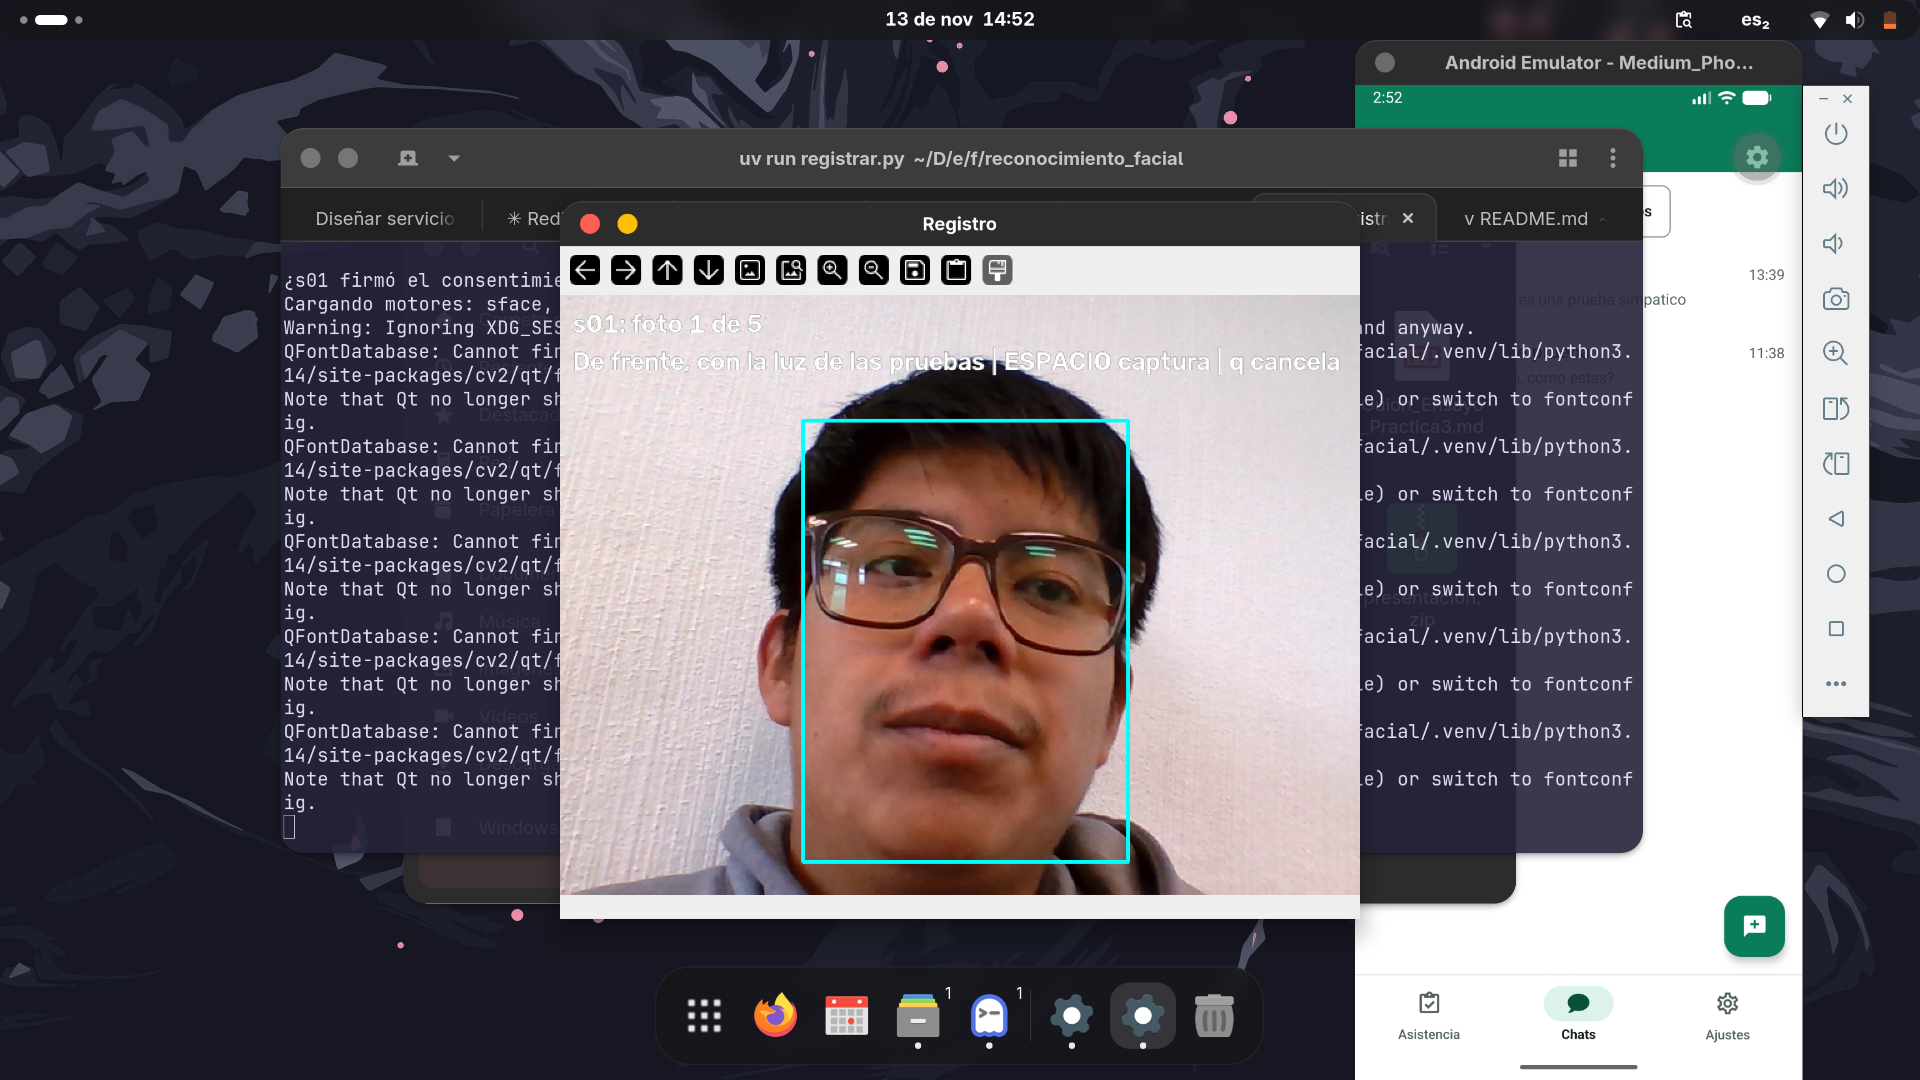
\includegraphics[width=\linewidth]{evidencias-2026-11-13/imagenes/01.png}
\end{center}
\figurenote{Captura del 13 de noviembre de 2026 a las 14:52:08. Se observa la ventana de registro, el encuadre de un rostro y la terminal del programa. La captura evidencia el procedimiento de registro; por sí sola no prueba que se hayan completado las cinco muestras ni que se hayan guardado todos los motores.}

El recuadro permite observar la detección del rostro durante el registro. La conclusión del proceso requiere verificar que se hayan guardado los vectores y asociado con el código del participante.

\clearpage
\subsection{Rechazo de una fotografía en un celular}
\begin{center}
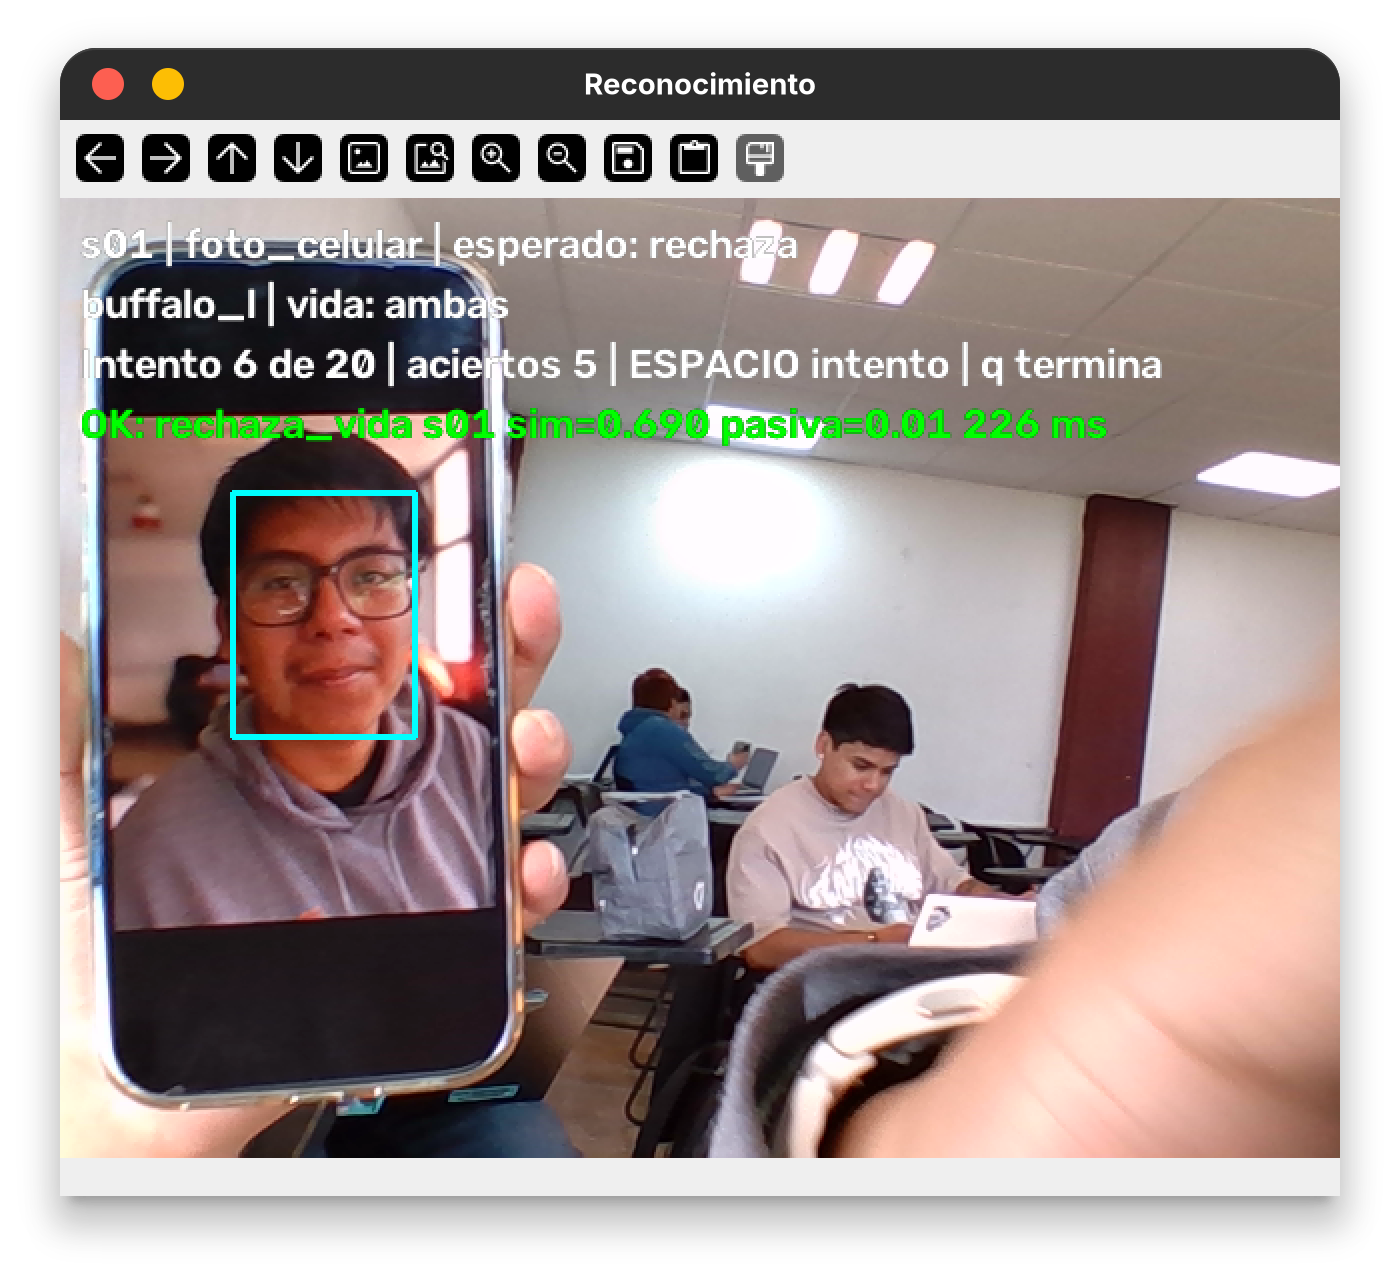
\includegraphics[height=16.5cm,width=\linewidth,keepaspectratio]{evidencias-2026-11-13/imagenes/02.png}
\end{center}
\figurenote{Captura del 13 de noviembre de 2026 a las 15:59:55. La pantalla indica s01, foto en celular, esperado rechazo y vida ambas. La última decisión visible es \texttt{rechaza\_vida}, similitud aproximada 0,690, puntaje pasivo 0,01 y 226 ms. Coincide con los valores del registro de las 15:59:39; la captura puede tomarse después de la decisión.}

Este resultado visual de rechazo debe leerse junto con los ocho intentos de la condición: el CSV también contiene la aceptación incorrecta de las 16:00:10. Una captura de éxito no sustituye el resumen completo.

\clearpage
\subsection{Aceptación con identidad distinta: primera captura}
\begin{center}
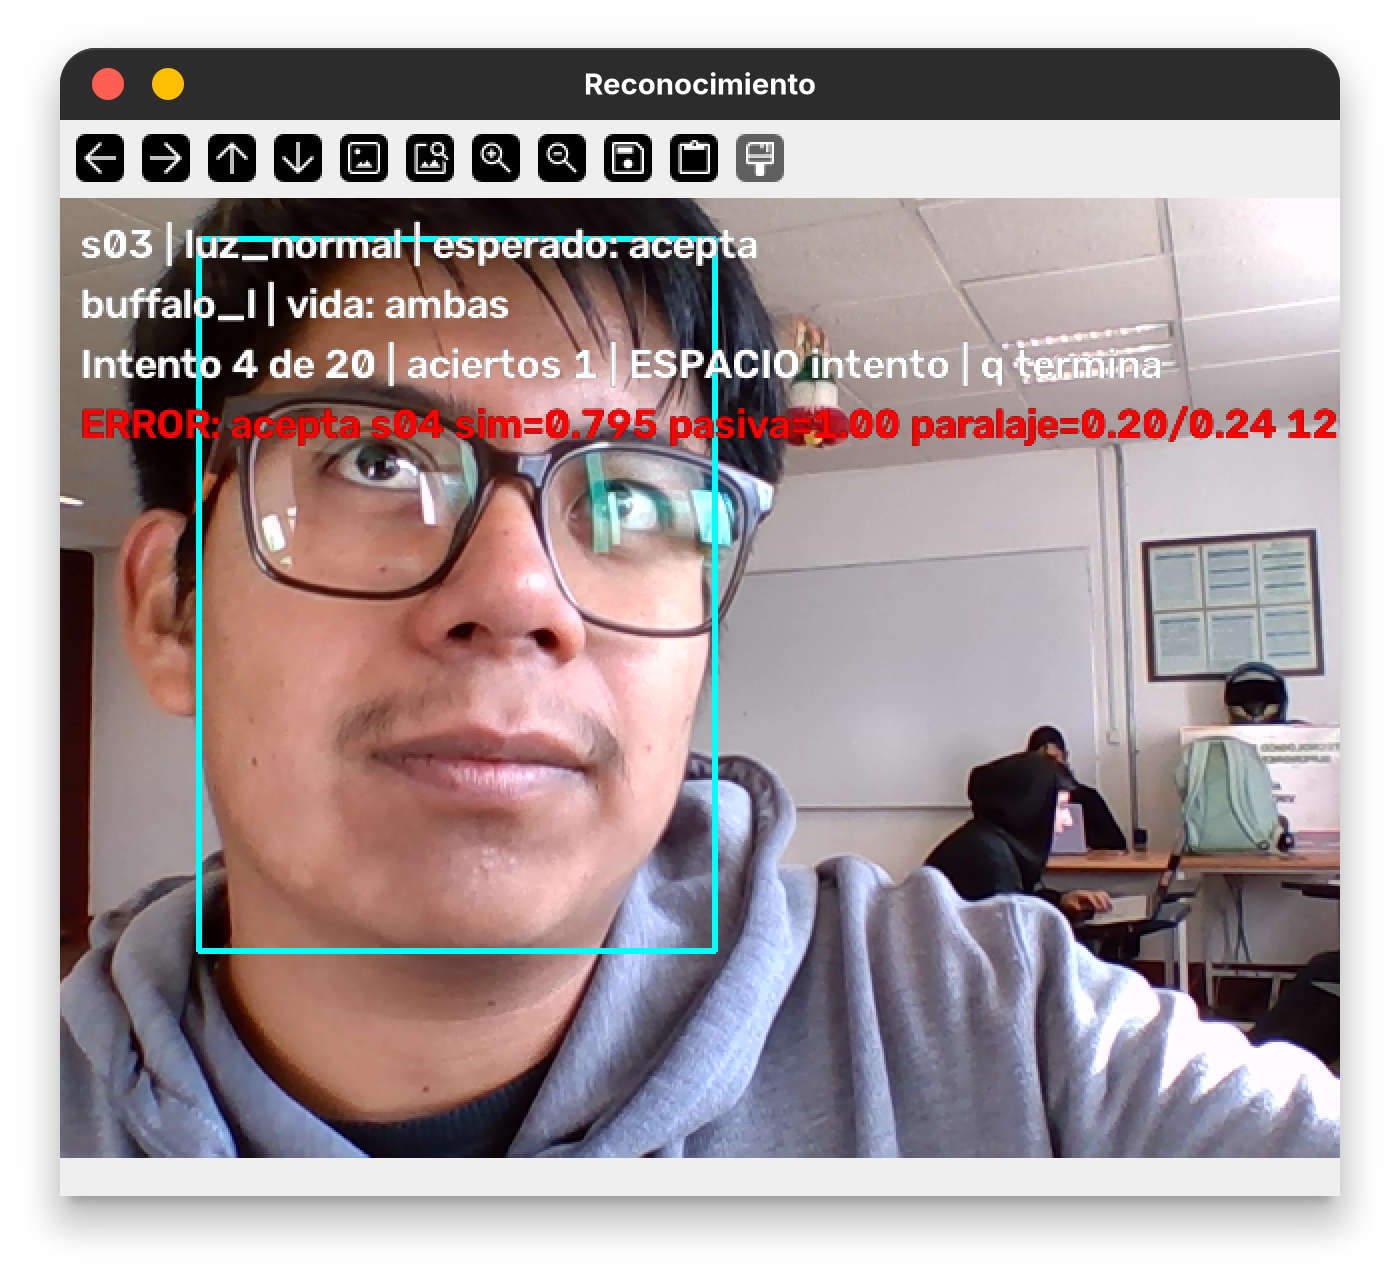
\includegraphics[height=16.5cm,width=\linewidth,keepaspectratio]{evidencias-2026-11-13/imagenes/03.png}
\end{center}
\figurenote{Captura del 13 de noviembre de 2026 a las 16:02:21. El encabezado indica s03 y esperado aceptación. En rojo, la interfaz conserva \texttt{ERROR: acepta s04}, similitud aproximada 0,795, vida pasiva 1,00 y paralaje 0,20/0,24. Es consistente con la decisión guardada a las 16:02:00.}

La prueba de vida no verifica que la etiqueta del participante sea correcta ni que el vector corresponda al código esperado. La revisión debe distinguir identificación, vida y etiquetado de sesión. Esta evidencia no determina por sí sola cuál de esos componentes originó la discrepancia.

\clearpage
\subsection{Aceptación con identidad distinta: segunda captura}
\begin{center}
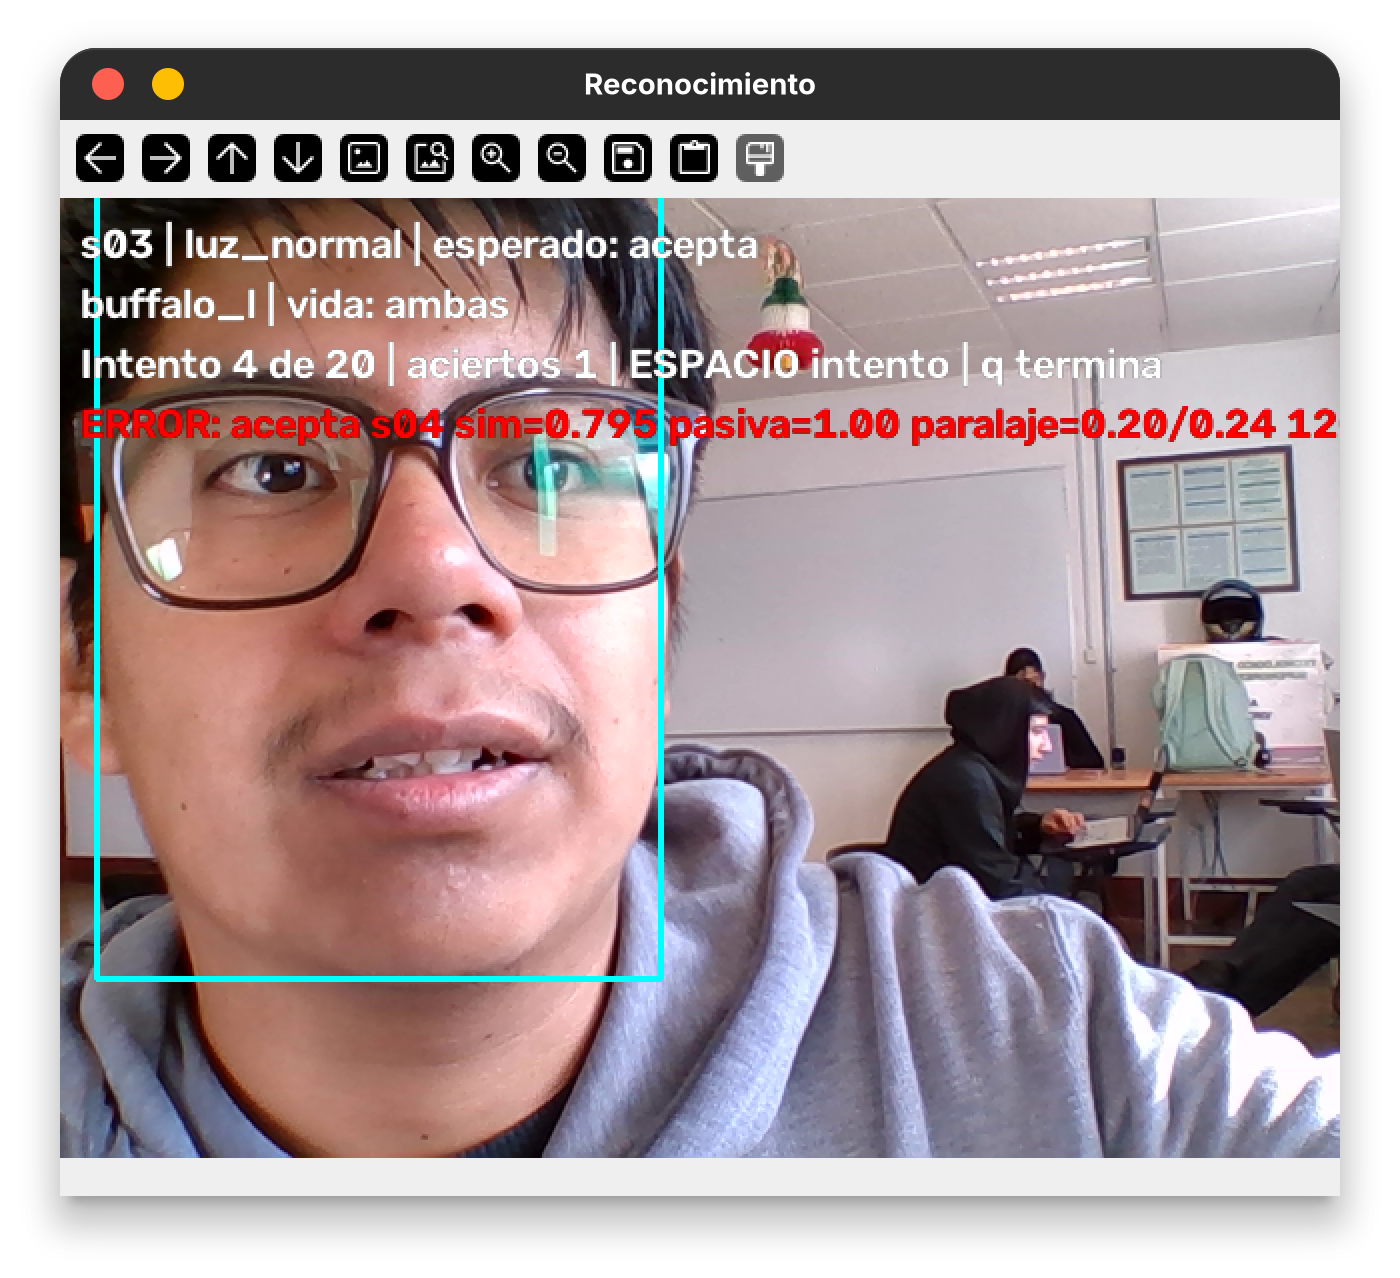
\includegraphics[height=16.5cm,width=\linewidth,keepaspectratio]{evidencias-2026-11-13/imagenes/04.png}
\end{center}
\figurenote{Captura del 13 de noviembre de 2026 a las 16:02:28. Conserva el encabezado de s03, el contador de intento 4 de 20 y la misma última decisión: aceptación como s04. Muestra que la última decisión permanece visible mientras continúa la vista de cámara, sin representar un intento adicional.}

Ambas capturas muestran el estado persistente de la interfaz entre intentos. Las repeticiones visibles de un resultado no se suman a los 24 registros; la marca de tiempo del CSV identifica el intento utilizado para el análisis.


\pagina{Catálogo de actividades del PERT original}
Las claves se conservan de la hoja compartida \parencite{pertEquipo}. La tabla siguiente sirve como diccionario para la red, el cálculo y la ruta de desarrollo.
\begin{longtable}{P{0.7cm}P{10.4cm}P{3.6cm}}
\toprule ID & Actividad & Responsable propuesto \\ \midrule
\endhead
A & Planteamiento del problema y pregunta de investigación & JEAC / equipo \\
B & Objetivos, justificación y metodología & JEAC / equipo \\
C & Diseño de encuesta, entrevista y hoja de observación & BUVR / equipo \\
D & Prueba de concepto facial: registro, reconocimiento y vida & IAFM / MAJD \\
E & Firmware ESP32-CAM como cámara de red & IAFM \\
F & Pruebas faciales de banco con voluntarios & BUVR / IAFM \\
G & Aplicación de encuesta y entrevistas & BUVR / equipo \\
H & Observación de línea base del acceso piloto & BUVR / equipo \\
I & Requisitos de protección de datos & MAJD / JEAC \\
J & Análisis del diagnóstico y requisitos del sistema & BUVR / JFRA \\
K & Arquitectura y diseño de la base de datos & MAJD / JFRA \\
L & Generación y validación de QR dinámicos con HMAC & MAJD \\
M & Base de datos de ingresos y panel web & JFRA \\
N & Firmware del lector QR en el ESP32-CAM & IAFM \\
O & Torniquete y controlador ESP32 & DAP \\
P & Pruebas de vencimiento, repetición, alteración y reloj & MAJD / BUVR \\
Q & Integración de lector, torniquete, servidor y panel & Equipo \\
R & Verificación técnica: tiempo, luz, brillo y distancia & BUVR / equipo \\
S & Comparación en banco entre facial, QR y NFC & BUVR / IAFM \\
T & Autorización para instalar el prototipo & JEAC \\
U & Piloto con observación en el acceso & BUVR / equipo \\
V & Evaluación: línea base frente al piloto & BUVR / JFRA \\
W & Informe final y recomendación & JEAC / equipo \\
\bottomrule
\end{longtable}
\tablenote{Las actividades provienen de la hoja; la asignación por actividad es una propuesta basada en los roles del documento de gestión. Debe confirmarse, especialmente para facial y NFC.}

\pagina{Estimaciones PERT y revisión de totales}
La hoja define tres estimaciones por tarea: optimista $a$, más probable $m$ y pesimista $b$, en días hábiles. Se recalculan las duraciones esperadas y la varianza con el esquema PERT clásico \parencite{cmuPert}:
\[
t_e=\frac{a+4m+b}{6},\qquad \sigma=\frac{b-a}{6},\qquad \sigma^2=\frac{(b-a)^2}{36}.
\]
\begin{center}\small\singlespacing
\begin{tabular}{lP{2.2cm}rrrrr}\toprule ID & Predecesoras & $a$ & $m$ & $b$ & $t_e$ & $\sigma^2$ \\ \midrule
A & -- & 3 & 5 & 8 & 5,17 & 0,69 \\
B & A & 3 & 5 & 8 & 5,17 & 0,69 \\
C & B & 2 & 4 & 6 & 4,00 & 0,44 \\
D & A & 2 & 4 & 7 & 4,17 & 0,69 \\
E & D & 1 & 2 & 5 & 2,33 & 0,44 \\
F & D, E & 2 & 3 & 5 & 3,17 & 0,25 \\
G & C & 3 & 5 & 8 & 5,17 & 0,69 \\
H & C & 5 & 5 & 7 & 5,33 & 0,11 \\
I & B & 2 & 3 & 6 & 3,33 & 0,44 \\
J & G, H & 2 & 3 & 5 & 3,17 & 0,25 \\
K & I, J & 3 & 5 & 8 & 5,17 & 0,69 \\
L & K & 4 & 6 & 10 & 6,33 & 1,00 \\
M & K & 4 & 7 & 11 & 7,17 & 1,36 \\
N & E, K & 4 & 7 & 12 & 7,33 & 1,78 \\
O & K & 5 & 8 & 14 & 8,50 & 2,25 \\
P & L & 1 & 2 & 4 & 2,17 & 0,25 \\
Q & M, N, O, P & 3 & 5 & 9 & 5,33 & 1,00 \\
R & Q & 2 & 3 & 5 & 3,17 & 0,25 \\
S & F, R & 2 & 3 & 6 & 3,33 & 0,44 \\
T & K & 3 & 5 & 10 & 5,50 & 1,36 \\
U & R, T & 5 & 5 & 7 & 5,33 & 0,11 \\
V & U & 2 & 3 & 5 & 3,17 & 0,25 \\
W & S, V & 3 & 4 & 7 & 4,33 & 0,44 \\
\midrule \multicolumn{5}{l}{Suma de las 23 actividades} & 107,83 & 15,92 \\ \bottomrule\end{tabular}
\end{center}
\tablenote{Fuente: estimaciones y dependencias del plan PERT del equipo; cálculos sin redondeo intermedio y presentación a dos decimales. No se usa el PERT mostrado a un decimal para encadenar las tareas.}

\subsection{Diferencias con la fila Total}
La hoja muestra 98 días en Tiempo, 103,5 en PERT y 15,9 en Varianza. Al sumar A a W se obtienen 102 días de tiempos más probables, 107,83 de tiempos esperados y 15,92 de varianzas. Las diferencias en Tiempo y PERT corresponden a W: 4 días y 4,33 días esperados. El total visible de varianza sí coincide al redondear a un decimal. Conviene revisar que los totales incluyan las 23 actividades y que la suma de varianzas considere únicamente las actividades, sin volver a incluir el total.

Sumar desviaciones estándar no produce la desviación del proyecto. Tampoco la suma de varianzas de todas las ramas es la varianza de una ruta. La planificación temporal depende de la red y de sus convergencias.

\pagina{Dependencias y red del proyecto}
Se interpreta cada relación de la hoja como \textbf{fin a inicio, sin desfase}: una tarea espera a todas sus predecesoras. Las ramas avanzan en paralelo si cuentan con recursos. La figura representa todas las dependencias, con inicio en A y fin en W.
\begin{center}
\textbf{Definición, exploración y diagnóstico}\par\medskip
\begin{tikzpicture}[x=1cm,y=1cm,box/.style={draw=azul,fill=suave,rounded corners,minimum width=0.8cm,minimum height=0.55cm,font=\small},arr/.style={-{Latex[length=1.6mm]},thin,azul}]
\node[box](A) at (0,0){A};\node[box](B) at (2,0){B};\node[box](C) at (4,0){C};
\node[box](D) at (2,2){D};\node[box](E) at (4,2){E};\node[box](F) at (6,2){F};
\node[box](G) at (6,0.65){G};\node[box](H) at (6,-0.65){H};\node[box](I) at (6,-2){I};\node[box](J) at (8,0){J};\node[box](K) at (10,0){K};
\foreach \s/\t in {A/B,B/C,A/D,D/E,E/F,C/G,C/H,G/J,H/J,I/K,J/K}{\draw[arr](\s)--(\t);}
\draw[arr](D.north)--++(0,0.6)-|(F.north);
\draw[arr](B.south)|-(I.west);
\end{tikzpicture}

\medskip\textbf{Construcción, integración y evaluación}\par\medskip
\begin{tikzpicture}[x=1cm,y=1cm,box/.style={draw=azul,fill=suave,rounded corners,minimum width=0.8cm,minimum height=0.55cm,font=\small},arr/.style={-{Latex[length=1.6mm]},thin,azul}]
\node[box](K) at (0,0){K};\node[box](L) at (2,2){L};\node[box](P) at (4,2){P};
\node[box](M) at (4,0.7){M};\node[box](N) at (4,-0.7){N};\node[box](O) at (4,-2){O};\node[box](E) at (2,-0.7){E};
\node[box](T) at (2,-3.2){T};\node[box](Q) at (6,0){Q};\node[box](R) at (8,0){R};
\node[box](F) at (8,2){F};\node[box](S) at (10,2){S};\node[box](U) at (10,-2){U};\node[box](V) at (12,-2){V};\node[box](W) at (13,0){W};
\foreach \s/\t in {K/L,L/P,K/M,K/N,E/N,K/T,M/Q,N/Q,O/Q,P/Q,Q/R,F/S,R/S,R/U,T/U,U/V,S/W,V/W}{\draw[arr](\s)--(\t);}
\draw[arr](K.west)--++(-0.6,0)|-(O.west);
\end{tikzpicture}
\end{center}
\figurenote{Los nodos E, F y K se repiten como puntos de conexión entre los dos paneles. Todas las dependencias corresponden a la hoja; la posición de un nodo no representa su fecha.}

\subsection{Condiciones externas no representadas como tareas}
La observación, las encuestas y las pruebas con voluntarios requieren acuerdos de acceso y tratamiento de datos antes de comenzar. La actividad T autoriza instalar el prototipo, pero no representa todos esos permisos. Deben registrarse como condiciones de entrada de F, G y H o incorporarse a una futura revisión del PERT.

S requiere hardware y programa NFC que no figuran como desarrollo previo en la red. E corresponde a cámara de red y N a lector QR: se debe decidir cómo se cambia el firmware o si se dispone de placas distintas. Comprar componentes, conseguir alimentación y comprobar la red también condicionan N, O y Q aunque no aparezcan como nodos independientes.

\pagina{Cálculo de precedencias, holguras y rutas críticas}
El recorrido hacia adelante obtiene inicio temprano (ES) y fin temprano (EF); el recorrido hacia atrás obtiene inicio tardío (LS) y fin tardío (LF). La holgura total es $LS-ES$. El origen lógico es el instante 0, sin fecha de calendario ni avance real descontado.
\[
ES_i=\max_{j\in pred(i)} EF_j,\quad EF_i=ES_i+t_{e,i},\quad
LF_i=\min_{k\in suc(i)}LS_k,\quad LS_i=LF_i-t_{e,i}.
\]
\begin{center}\small\singlespacing
\begin{tabular}{lrrrrrl}\toprule ID & ES & EF & LS & LF & Holgura & Crítica \\ \midrule
A & 0,00 & 5,17 & 0,00 & 5,17 & 0,00 & Sí \\
B & 5,17 & 10,33 & 5,17 & 10,33 & 0,00 & Sí \\
C & 10,33 & 14,33 & 10,33 & 14,33 & 0,00 & Sí \\
D & 5,17 & 9,33 & 22,67 & 26,83 & 17,50 & No \\
E & 9,33 & 11,67 & 26,83 & 29,17 & 17,50 & No \\
F & 11,67 & 14,83 & 47,00 & 50,17 & 35,33 & No \\
G & 14,33 & 19,50 & 14,50 & 19,67 & 0,17 & No \\
H & 14,33 & 19,67 & 14,33 & 19,67 & 0,00 & Sí \\
I & 10,33 & 13,67 & 19,50 & 22,83 & 9,17 & No \\
J & 19,67 & 22,83 & 19,67 & 22,83 & 0,00 & Sí \\
K & 22,83 & 28,00 & 22,83 & 28,00 & 0,00 & Sí \\
L & 28,00 & 34,33 & 28,00 & 34,33 & 0,00 & Sí \\
M & 28,00 & 35,17 & 29,33 & 36,50 & 1,33 & No \\
N & 28,00 & 35,33 & 29,17 & 36,50 & 1,17 & No \\
O & 28,00 & 36,50 & 28,00 & 36,50 & 0,00 & Sí \\
P & 34,33 & 36,50 & 34,33 & 36,50 & 0,00 & Sí \\
Q & 36,50 & 41,83 & 36,50 & 41,83 & 0,00 & Sí \\
R & 41,83 & 45,00 & 41,83 & 45,00 & 0,00 & Sí \\
S & 45,00 & 48,33 & 50,17 & 53,50 & 5,17 & No \\
T & 28,00 & 33,50 & 39,50 & 45,00 & 11,50 & No \\
U & 45,00 & 50,33 & 45,00 & 50,33 & 0,00 & Sí \\
V & 50,33 & 53,50 & 50,33 & 53,50 & 0,00 & Sí \\
W & 53,50 & 57,83 & 53,50 & 57,83 & 0,00 & Sí \\
\bottomrule\end{tabular}
\end{center}
\tablenote{Valores calculados a partir de las estimaciones del plan PERT y sus dependencias originales. Todas las cantidades son días hábiles; dos decimales solo para presentación.}

El camino más largo hasta W dura \textbf{57,83 días}. G dispone de apenas 0,17 días de holgura; M y N tienen 1,33 y 1,17. Aunque no sean críticas en este cálculo, son sensibles a retrasos. El trabajo compartido por responsables puede consumir esas holguras; el CPM no nivela automáticamente la capacidad del equipo.

\pagina{Dos rutas críticas y orden temporal}
Hay dos rutas con igual duración esperada porque la rama O y la secuencia L--P llegan a Q en el mismo instante:
\begin{quote}
\textbf{Ruta 1:} A $\rightarrow$ B $\rightarrow$ C $\rightarrow$ H $\rightarrow$ J $\rightarrow$ K $\rightarrow$ O $\rightarrow$ Q $\rightarrow$ R $\rightarrow$ U $\rightarrow$ V $\rightarrow$ W.

\textbf{Ruta 2:} A $\rightarrow$ B $\rightarrow$ C $\rightarrow$ H $\rightarrow$ J $\rightarrow$ K $\rightarrow$ L $\rightarrow$ P $\rightarrow$ Q $\rightarrow$ R $\rightarrow$ U $\rightarrow$ V $\rightarrow$ W.
\end{quote}
En ambas, la duración es 57,83 días. O tiene duración 8,50 y L más P suma 8,50. No se deben escribir O, L y P como una secuencia única ni sumar las duraciones de todos los nodos críticos: son ramas paralelas.

\begin{center}\begin{tikzpicture}[x=0.24cm,y=-0.40cm,font=\scriptsize]
\draw[gray!20] (0,0) -- (0,23.8);\node[above] at (0,0) {0};
\draw[gray!20] (5,0) -- (5,23.8);\node[above] at (5,0) {5};
\draw[gray!20] (10,0) -- (10,23.8);\node[above] at (10,0) {10};
\draw[gray!20] (15,0) -- (15,23.8);\node[above] at (15,0) {15};
\draw[gray!20] (20,0) -- (20,23.8);\node[above] at (20,0) {20};
\draw[gray!20] (25,0) -- (25,23.8);\node[above] at (25,0) {25};
\draw[gray!20] (30,0) -- (30,23.8);\node[above] at (30,0) {30};
\draw[gray!20] (35,0) -- (35,23.8);\node[above] at (35,0) {35};
\draw[gray!20] (40,0) -- (40,23.8);\node[above] at (40,0) {40};
\draw[gray!20] (45,0) -- (45,23.8);\node[above] at (45,0) {45};
\draw[gray!20] (50,0) -- (50,23.8);\node[above] at (50,0) {50};
\draw[gray!20] (55,0) -- (55,23.8);\node[above] at (55,0) {55};
\draw[gray!20] (60,0) -- (60,23.8);\node[above] at (60,0) {60};
\node[anchor=east] at (-0.4,1) {A};\fill[critico] (0.0,0.77) rectangle (5.166666666666667,1.23);
\node[anchor=east] at (-0.4,2) {B};\fill[critico] (5.166666666666667,1.77) rectangle (10.333333333333334,2.23);
\node[anchor=east] at (-0.4,3) {C};\fill[critico] (10.333333333333334,2.77) rectangle (14.333333333333334,3.23);
\node[anchor=east] at (-0.4,4) {D};\fill[azul] (5.166666666666667,3.77) rectangle (9.333333333333334,4.23);
\node[anchor=east] at (-0.4,5) {E};\fill[azul] (9.333333333333334,4.77) rectangle (11.666666666666666,5.23);
\node[anchor=east] at (-0.4,6) {F};\fill[azul] (11.666666666666666,5.77) rectangle (14.833333333333334,6.23);
\node[anchor=east] at (-0.4,7) {G};\fill[azul] (14.333333333333334,6.77) rectangle (19.5,7.23);
\node[anchor=east] at (-0.4,8) {H};\fill[critico] (14.333333333333334,7.77) rectangle (19.666666666666668,8.23);
\node[anchor=east] at (-0.4,9) {I};\fill[azul] (10.333333333333334,8.77) rectangle (13.666666666666666,9.23);
\node[anchor=east] at (-0.4,10) {J};\fill[critico] (19.666666666666668,9.77) rectangle (22.833333333333332,10.23);
\node[anchor=east] at (-0.4,11) {K};\fill[critico] (22.833333333333332,10.77) rectangle (28.0,11.23);
\node[anchor=east] at (-0.4,12) {L};\fill[critico] (28.0,11.77) rectangle (34.333333333333336,12.23);
\node[anchor=east] at (-0.4,13) {M};\fill[azul] (28.0,12.77) rectangle (35.166666666666664,13.23);
\node[anchor=east] at (-0.4,14) {N};\fill[azul] (28.0,13.77) rectangle (35.333333333333336,14.23);
\node[anchor=east] at (-0.4,15) {O};\fill[critico] (28.0,14.77) rectangle (36.5,15.23);
\node[anchor=east] at (-0.4,16) {P};\fill[critico] (34.333333333333336,15.77) rectangle (36.5,16.23);
\node[anchor=east] at (-0.4,17) {Q};\fill[critico] (36.5,16.77) rectangle (41.833333333333336,17.23);
\node[anchor=east] at (-0.4,18) {R};\fill[critico] (41.833333333333336,17.77) rectangle (45.0,18.23);
\node[anchor=east] at (-0.4,19) {S};\fill[azul] (45.0,18.77) rectangle (48.333333333333336,19.23);
\node[anchor=east] at (-0.4,20) {T};\fill[azul] (28.0,19.77) rectangle (33.5,20.23);
\node[anchor=east] at (-0.4,21) {U};\fill[critico] (45.0,20.77) rectangle (50.333333333333336,21.23);
\node[anchor=east] at (-0.4,22) {V};\fill[critico] (50.333333333333336,21.77) rectangle (53.5,22.23);
\node[anchor=east] at (-0.4,23) {W};\fill[critico] (53.5,22.77) rectangle (57.833333333333336,23.23);
\end{tikzpicture}
\end{center}
\figurenote{Gantt relativo de inicios tempranos. Eje horizontal: días hábiles desde el inicio lógico. Rojo: actividades con holgura cero; gris: actividades con holgura positiva. No representa trabajo efectivamente realizado.}

Si se supone independencia de tiempos, la varianza de la ruta 1 es 7,19 días cuadrados y su desviación 2,68 días; en la ruta 2 son 6,19 y 2,49. Son cálculos por ruta. La convergencia de ramas y los recursos compartidos impiden usarlos como una probabilidad validada de entrega. Un retraso en cualquiera de las dos ramas críticas puede desplazar Q y el cierre.

\pagina{Calendario original y trabajo restante}
\subsection{Hitos documentados}
El documento de gestión fija planeación del 5 al 16 de octubre, diagnóstico del 12 al 30 de octubre, desarrollo del 26 de octubre al 27 de noviembre, pruebas y piloto hasta el 18 de diciembre, y cierre del 4 al 29 de enero de 2027. Las semanas del 21 y 28 de diciembre se reservan como vacaciones. Estas son fechas del plan original, no fechas reales verificadas de terminación.

El PERT consultado no fija una fecha de inicio, porcentajes de avance ni fechas reales. Los 57,83 días corresponden a la red completa desde A. No deben contarse de nuevo desde noviembre si A, B u otras tareas ya se cerraron, ni descontarse automáticamente porque la hoja diga que tienen avance.

\subsection{Escenario condicional desde el corte}
Si el equipo confirma que \textbf{A a F están terminadas}, que G a W están pendientes y que no hay trabajo residual ni restricciones adicionales, la red restante tiene una duración esperada de \textbf{43,50 días hábiles}. Este escenario se calcula poniendo a cero la duración pendiente de A a F, manteniendo las dependencias y las otras estimaciones. No constituye una certificación de avance.

Como referencia, del 16 de noviembre de 2026 al 29 de enero de 2027 hay 45 jornadas de lunes a viernes si se excluye únicamente el receso del 21 de diciembre al 1 de enero. Bajo esa convención quedarían solo 1,50 jornadas de margen frente al escenario restante. El conteo todavía debe ajustarse a días inhábiles, calendario del plantel, disponibilidad de observadores, permisos y dedicación real. Por ello no se asigna aquí una fecha de entrega comprometida.

Con esas hipótesis, no queda sustentado conservar el piloto de diciembre: su término temprano sería a los 36 días hábiles de trabajo restante, mientras que antes del receso solo hay 25 jornadas en esa referencia. Se requiere reprogramar el piloto o revisar duraciones, alcance y recursos con evidencia.

\subsection{Cómo actualizar el calendario}
Confirmar cierres con evidencias; capturar trabajo restante por actividad en curso; fijar calendario oficial y disponibilidad por persona; añadir permisos, compras y NFC si corresponde; recalcular precedencias y nivelar recursos. Registrar la versión resultante como nueva línea base, conservando la original para comparar variaciones.

\pagina{Ruta de desarrollo por entregables}
La ruta práctica usa las claves del PERT y separa el avance documental del cierre técnico. El equipo puede trabajar en paralelo después de K, pero la integración Q espera a M, N, O y P.
\begin{longtable}{P{1.5cm}P{5cm}P{8cm}}
\toprule Etapa & Actividades & Evidencia para avanzar \\ \midrule
\endhead
1 & A, B y C: consolidar definición e instrumentos & Problema y objetivos consistentes, alcance QR explícito y formatos de encuesta, entrevista y observación revisados. \\[0.4em]
2 & D, E, F e I: cerrar exploración y requisitos & Código y configuración facial identificados; prueba de cámara de red; resultados trazables; reglas de acceso y datos definidas antes de trabajar con personas. \\[0.4em]
3 & G, H y J: diagnosticar & Instrumentos aplicados; cinco días de línea base; datos depurados; necesidades de usuarios y restricciones del acceso. \\[0.4em]
4 & K: diseñar integración & Diagrama de componentes, modelo de datos, formato del QR y contrato de mensajes de validación, errores y apertura. Decisión sobre firmware y equipo. \\[0.4em]
5 & L y P: construir validación & Generación de QR; validación de firma, vigencia, repetición y reloj; casos de prueba reproducibles y registros. \\[0.4em]
6 & M, N y O: completar frentes & Base de datos, página del estudiante y panel; lector real con mensajes de prueba; torniquete de banco con alimentación y control verificados. \\[0.4em]
7 & Q y R: integrar y medir & Un intento completo aceptado, uno rechazado y un reintento sin doble apertura; matriz de luz, brillo y distancia con tiempos y fallos. \\[0.4em]
8 & S, T y U: comparar y pilotar & NFC disponible si se conserva S; autorización de instalación; revisión manual disponible; observación equivalente durante cinco días del piloto. \\[0.4em]
9 & V y W: interpretar y entregar & Comparación de indicadores, límites de interpretación, código, manual, evidencias y recomendación final. \\
\bottomrule
\end{longtable}
\tablenote{Las etapas ordenan el trabajo; no reemplazan las predecesoras exactas de la red. Las condiciones de entrada de privacidad y permisos complementan la hoja.}

\pagina{Contratos de integración y modelo de datos}
\subsection{Acuerdos que debe producir K}
El diseño debe fijar quién emite el token, quién conserva los secretos, qué dispositivo valida, cuánto dura la vigencia y cómo se informa el motivo de rechazo. También debe definir comportamiento ante desconexión, petición duplicada, reinicio del lector, servidor sin respuesta y mecanismo que no confirma su movimiento. Las decisiones se documentan antes de programar cada frente.

\subsection{Datos mínimos propuestos}
\begin{longtable}{P{3.5cm}P{11.3cm}}
\toprule Entidad & Contenido y regla principal \\ \midrule
\endhead
Estudiante & Identificador interno, estado de autorización y datos mínimos acordados. Una baja debe impedir nuevos accesos sin borrar indebidamente la trazabilidad que se haya autorizado conservar. \\[0.4em]
Dispositivo & Identificador, acceso asociado y credencial técnica. Distinguir un lector autorizado de una petición arbitraria. \\[0.4em]
Emisión o uso de token & Identificador único, estudiante, vigencia y estado de consumo. Definir una operación atómica para evitar dos aceptaciones simultáneas. \\[0.4em]
Intento de acceso & Identificador de intento, fecha, dispositivo, resultado, motivo e identificador de autorización, si existe. El reintento del mismo mensaje no crea un ingreso nuevo. \\[0.4em]
Cuenta del personal & Identidad y permisos de consulta o administración. Separar la administración de estudiantes de la consulta de registros. \\[0.4em]
Sesión de pruebas & Código de sesión, participante seudonimizado, condiciones, versiones y configuración. Mantenerla separada de los registros operativos. \\ \bottomrule
\end{longtable}
\tablenote{Modelo conceptual propuesto a partir de los objetivos. Todavía no es un esquema de base de datos implementado.}

\subsection{Mensajes de entrada y salida}
Como propuesta de contrato, el lector envía identificador de dispositivo e intento y el token leído. La respuesta contiene el mismo identificador de intento, decisión, motivo y una autorización de apertura única cuando corresponde. El controlador confirma si pudo ejecutar la orden. Los tiempos límite, formatos y transporte deben definirse en K; no se encontró una API existente que permita fijarlos como hechos.

La biometría permanecerá fuera de las tablas operativas del piloto QR. Si se decide integrarla posteriormente, habrá que definir para qué se usa, cómo cambia la autorización y cómo se verifica esa nueva conducta.

\pagina{Plan de pruebas y criterios de salida}
\begin{longtable}{P{2.8cm}P{6.1cm}P{5.9cm}}
\toprule Grupo & Casos mínimos & Evidencia de aceptación \\ \midrule
\endhead
QR y servidor (L, P) & Válido, vencido, alterado, repetido, estudiante inhabilitado, reloj desfasado y dos solicitudes simultáneas. & Tabla de entrada, resultado esperado y obtenido. Todos los casos negativos definidos se rechazan; el válido se registra una vez. \\[0.4em]
Lector y control (N, O) & Lectura, falla de cámara, pérdida de comunicación, reinicio, respuesta duplicada y orden fuera de vigencia. & Registro del banco y demostración del mecanismo sin apertura no autorizada o duplicada. \\[0.4em]
Integración (Q) & Alumno a lector, servidor, BD, controlador y panel; rechazo y reintento. & Un identificador trazable en todo el recorrido y correspondencia entre decisión, registro y movimiento. \\[0.4em]
Desempeño (R) & Combinaciones de luz, brillo y distancia; varias repeticiones con el mismo protocolo. & Tasa de lecturas exitosas y distribución de tiempos; metadatos de equipo y configuración. \\[0.4em]
Facial (F) & Titular, no registrado, poca luz, foto impresa, foto en celular y fallos del reto. & CSV por sesión y matriz de confusión por motor y vida; umbrales calibrados con conjuntos separados de evaluación. \\[0.4em]
Comparación (S) & Facial, QR y NFC bajo protocolo y recorrido de tiempo equivalentes. & Misma unidad de medición. Si falta una tecnología, declarar la comparación incompleta. \\[0.4em]
Campo (U, V) & Línea base y piloto con mismo acceso, turno, franja e instrumento. & Cinco días por etapa, con número de puntos de revisión y excepciones registrados; análisis de cambios y amenazas a la interpretación. \\ \bottomrule
\end{longtable}

El informe debe distinguir rechazo por identidad de rechazo por falta de rostro o falla técnica. El CSV actual permite marcar ambos como decisión no aceptada; para la evaluación se reportarán además como categorías separadas. La tasa de falsa aceptación se calcula sobre casos que debían rechazarse, y la de falso rechazo sobre casos que debían aceptarse.

El ingreso al piloto requiere permiso, prototipo integrado, casos de seguridad aprobados, respaldo manual y personal informado. Si falta alguna condición, se conserva la prueba en laboratorio y se actualiza el calendario.

\pagina{Equipo, recursos, presupuesto y riesgos}
\subsection{Responsabilidades documentadas}
JEAC coordina gestión y entregables; DAP atiende hardware; IAFM el lector; MAJD servidor y seguridad; JFRA datos y páginas web; BUVR campo y pruebas. Los seis colaboran en medición e integración. La asignación por actividad de este informe usa esos roles como propuesta, no como disponibilidad confirmada.

La programación temprana puede superponer tareas del mismo responsable: G con H; L con pruebas P; o medición de campo con comparaciones de banco. Debe verificarse capacidad antes de comprometer fechas. Las holguras calculadas pertenecen a la red lógica y no implican que una persona tenga ese tiempo libre.

\subsection{Presupuesto de referencia del documento de gestión}
\begin{center}
\begin{tabular}{P{10.5cm}r}
\toprule Concepto & Estimación (MXN) \\ \midrule
Hardware del prototipo & 1750 \\
Servidor, dominio y alojamiento por cuatro meses & 970 \\
Impresiones y material de campo & 600 \\
Traslados y compras & 400 \\
Reserva de contingencia & 380 \\
\midrule Total documentado & 4100 \\ \bottomrule
\end{tabular}
\end{center}
\tablenote{Presupuesto histórico preliminar, no cotización actual ni gasto ejercido. El subtotal es 3720; la reserva de 380 equivale aproximadamente al 10\,\%. NFC, reposiciones o ampliación facial deben cotejarse con el inventario. Las cerca de 800 horas de equipo mencionadas en gestión no se monetizan.}

\subsection{Riesgos que condicionan el desarrollo}
\begin{itemize}
\item \textbf{Permisos y datos:} gestionar condiciones antes de pruebas con personas; si no hay permiso de instalación, mantener banco de laboratorio. Responsable de seguimiento: JEAC con MAJD.
\item \textbf{Red y servidor:} definir fallos y reintentos. El modo fuera de línea mencionado en gestión no está implementado en la evidencia revisada y no debe suponerse disponible. MAJD e IAFM.
\item \textbf{Hardware y firmware:} confirmar componentes, alimentación y uso de la cámara; evitar que cambiar a video elimine el lector QR sin una configuración reproducible. DAP e IAFM.
\item \textbf{Calendario y recursos:} vigilar ambas rutas críticas y las holguras pequeñas; nivelar observadores y desarrolladores. JEAC.
\item \textbf{Comparación incompleta:} conseguir NFC o registrar un cambio de alcance de S y W; no presentar una comparación de tres tecnologías sin evidencia. BUVR.
\end{itemize}

\pagina{Seguimiento, entrega y siguientes acciones}
\subsection{Control del trabajo}
Revisar semanalmente el tablero de actividades A a W. Cada registro debe indicar estado, responsable, evidencia, bloqueo y estimación restante. Cuando cambie una dependencia o duración, recalcular la red, identificar ambas rutas críticas y registrar el efecto en el cierre. El avance se basa en productos aceptados; un retraso en permisos o suministro requiere una actualización explícita.

Se propone cerrar cada iteración con una demostración pequeña: token generado y rechazado correctamente; validación con registro; lector que consulta; apertura controlada; panel que recupera el mismo intento; flujo completo medido. Estas demostraciones hacen revisable la integración antes del piloto.

\subsection{Paquete de entrega}
\begin{enumerate}
\item Documento de investigación y diagnóstico, con instrumentos y resultados.
\item Código del servidor, página, panel, firmware y prototipo facial, con versiones y preparación del entorno.
\item Diseño de arquitectura, datos y contrato de integración, más inventario del hardware.
\item Prototipo de banco y evidencia de integración, incluyendo resultados negativos de seguridad.
\item PERT actualizado, red de dependencias, rutas críticas, calendario y bitácora de cambios.
\item Informe del piloto y comparación con la línea base; comparación tecnológica de banco con límites explícitos.
\item Manual de uso, manejo de fallas, política de acceso a datos y reglas de conservación o eliminación acordadas con el plantel.
\end{enumerate}

\subsection{Siguientes acciones concretas}
Primero, confirmar qué productos de A a F están cerrados y adjuntar sus evidencias, especialmente el firmware de E. Después, revisar los totales de la hoja y decidir si S conserva NFC; ambas decisiones afectan la interpretación del plan. A continuación, resolver permisos de campo y tratamiento de datos, aplicar o consolidar G y H y producir J. Con esos insumos, K fija arquitectura y contratos para abrir los frentes de desarrollo.

La siguiente versión del calendario deberá partir de ese estado real y de la capacidad de los seis integrantes. Mientras no se confirmen, los 57,83 días son la duración de la red completa y los 43,50 días son únicamente un escenario de trabajo restante condicionado.

\clearpage
\section{Referencias}
\printbibliography[heading=none]

\end{document}
